\chapter{Preface}
\addcontentsline{toc}{chapterdescription}{Why this book now? We describe how we came to write this book, and why now is the best time ever to build a world that works for you. You will read about Graham's and Jack's drivers and journeys, about how our climate grief has shaped both of us, and this book, from long before we met. Read this book in any way you want to; reading it in a circle, randomly starting anywhere, or even backwards. Whatever works best for you. (It's pretty good at keeping doors open.)}
\label{chapter:preface}




\begin{chapterquotation}
When you light a candle, you also cast a shadow.\\
\raggedleft\textemdash Ursula K. Le Guin\index{Le Guin, Ursula K.}
\end{chapterquotation}






\section*{Why this book now?}
As we finish this book in 2020, we both have more hope than when we met in 2015. Certainly more hope than Graham had when he left Procter and Gamble (P\&G)\index{Procter and Gamble} in 2008 to address the root causes. We have more hope because finally enough people are standing up and taking action to deal with the climate emergency, and all other global scale crises, that all of us are now in\cite{ten-signs-climate}. And because we now know how to rebuild our constructs of opposing elements, such as impact / regeneration or profit, into one complementary pairing: high impact \emph{and} high profit.


\begin{longstoryblock}
I (Graham) have had to fight for my hope, because my gut instinct, my intuition, has left me feeling hopeless over most of the past decade. At least we now have names for what many of us have experienced for over ten years: it’s variously called climate grief, climate depression, or climate anxiety. I remember clearly cycling in and out of climate depression in 2016 and 2017 watching the Arctic \index{Arctic} summer ice melt. The worst was mid-September 2017. I was completely unable to put my physical and mental trauma into coherent sentences; at home all I could do was point at the data and hope my partner would understand why even getting out of bed was an achievement. 
\end{longstoryblock}


And yet Jack and I both know that there are reasons to hope\index{hope}. We know that, paradoxically, because of the growing climate awareness, anxiety, and action, there has never been a better time to build the regenerative economy and the businesses that we need. So we have written this how-to book to describe why we believe that, how to look at yourself and your world, and what to do if you are committed to building a world that works for yourself, for others, and for nature. 


We can all transform how we come together as one human society of 8 billion unique individuals, the economy that our society constructs, how business works, and how each of us shows up in the world. Now is the best time ever to do that at a global scale, because we are so connected globally and have a greater understanding than ever before of all scales, from the individual to the planet. 


There have been times, though, when the two of us have felt anger or despair, not hope. In 2015, when we started this journey together, it was only a climate crisis, with 10 to 15 years left before the effects of climate change were experienced by many. We both imagined that within a few years enough people would start taking action. 


That didn't happen. Now we have a full-blown climate emergency, along with all our other interlinked social and environmental threats, and need immediate \emph{effective} global action; And the latest signals from our climate, society, and environment prove that the change is coming even faster and bigger than the original worst-case scenarios. So we urge everyone to act, put into practice now the proven approaches in this how-to guide. The more of us that do, the more hope we have. 


\begin{longstoryblock}
The central pillar in delivering radical change without going through a full-scale collapse of global systems is our growing understanding of how each of our individual identities, the identity of each group of people, along with our norms and global institutions, are our meaning-making stories made concrete.
\end{longstoryblock}


By going back to our meaning-making stories\index{meaning-making stories}, and transforming them, we have more power than ever before to change, at a fundamental level, everything that is part of our society, and our impact on each other and the planet.


There is hope\index{hope}. There is always hope. We intend this book to light a new candle of hope in you, perhaps even many new candles. A candle because you will see in this book one way of making business an intrinsic force for good, and creating a new kind of global economy that makes our lives better both today and in the future because it provides a multi-solution to our challenges.


This will only make a difference if each of us then turns that hope into action. Hope without right action is meaningless. 


Which begins and ends (as this book does) with a question both of us, and most likely you, have asked yourself before: \emph{“Who am I, and what am I for?”}




\section*{How we came to write this book together}


\subsection*{Graham}
One of my earliest memories is each morning crawling through a hole in the hedge that separated our house from the nursery school next door. Also, apparently, on the morning before I was born, my mom walked through the gate in the fence separating the house from the hospital, through the back door and straight into the maternity ward I was born in. (My dad was the hospital pharmacist.)


Maybe this tendency to ignore artificial boundaries, to go straight from one domain into another, was embedded into me at birth.


Or maybe it's something that I grew into, growing up in apartheid South Africa\index{South Africa} and seeing how arbitrary and harmful many of the boundaries\index{boundaries} were. All my life I've wanted to understand why things are the way they are. Early on, that took me into taking apart then trying to put back together everything I could lay my hands on. I learnt that that didn't always (in fact, rather seldom) end up with all the parts fitting together and working the way they had done before.


I have always been a voracious reader of all kinds of books about how the physical world and how human beings work. The cognitive behavioural approaches in psychology were interesting, and helped me hold steady in the face of repeated bouts of depression. I recall beginning to read about climate change, and the limits to growth, in the early 80s, and thought then that this would happen only at the very end of my life.


I went to a highly competitive all boys school, Selborne. Mathematics and physics became my focus; and I was encouraged to find and compete in a sport that suited me. Rowing ended up as that sport. Later on at university I complemented rowing with hiking and climbing on Table Mountain.


This competitive edge has stayed with me ever since, a curse and a blessing. It drives me to always try harder, take on the toughest challenges I can find; and keeps me constantly judging myself as not good enough. It's still with me, only now I know that none of us can possibly be individually good enough for the challenges we are facing.


I dived ever deeper into theoretical physics, getting my PhD in Germany (J\"ulich and Bielefeld), and researching high-temperature particle physics in Pisa (Italy), and Tsukuba (Japan). By Tsukuba I was starting to think that it was time to do something completely new, so I accepted a job offer as R\&D manager with P\&G in Belgium. Four years later P\&G decided that I would be a good person to lead the packaging unit in the R\&D centre in Beijing, and so I moved to China.


I was also beginning to panic, looking at how fast humanity was heading towards multiple crises. 


So in 2008 I left P\&G\index{Procter and Gamble}. The Arctic\index{Arctic} ice data, and everything else, were unambiguous: by 2020 we would all experience physical consequences of the climate crisis. It was perfectly clear to me: now was the time for decisive, global action to address climate change. I found it hard to grasp how few of my friends, family, and colleagues had any sense of fear about the future. I found it hard to believe that most of the people I talked to expected the money they were putting into pension funds to still be worth something in their last years of retirement. I certainly didn't.


We clearly had just 15 to 25 years to take decisive regenerative action. But what would actually be regenerative action, rather than the degenerative action driven by blame and anger, rooted in powerlessness, from a meaning\hyp{} akin to hoping for a different past, as Desmond Tutu \index{Tutu, Desmond} puts it?


By 2008 the hard data had become crystal clear. We had entered the endgame of life in a climate suited to humans, with \emph{at most} a mere two decades to take decisive action. Despite first being warned as far back as 1856 by Eunice Newton Foote\cite{foote-greenhouse-gas}\index{Foote, Eunice Newton} that carbon dioxide was a blanket keeping the Earth cosy enough for our comfortable life, and that increasing CO$_2$ adds blankets. Three years later the first oil well was drilled, and we began adding blankets. 


\begin{figure}
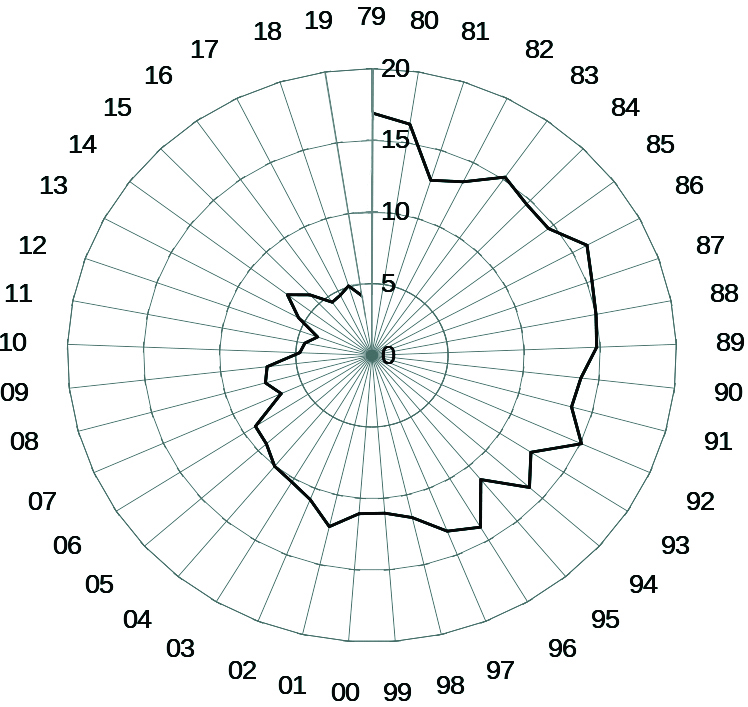
\includegraphics[width=0.50\textwidth]{./Images/arctic-death-spiral}
\caption[Arctic ice death spiral]{Plotted here is the Arctic ice volume\cite{piomas-data} each year from 1979 to 2019 at the September minimum, after the summer melt, in 1000km$^3$. As you can see, it is spiralling inexorably in, towards zero arctic ice in summer. Which will turn the mild European winters into freezing, because the Gulf stream will weaken.}
\label{fig:arctic-death-spiral}
\end{figure}


The Arctic\index{Arctic} death spiral shown in Figure~\ref{fig:arctic-death-spiral} was the clincher, and everything I have seen since then confirms that we humans consistently under-estimate how fast the climate emergency is growing. Most significantly, a few weeks before we finished final editing, a new computer simulation from Maria-Vittoria Guarino\index{Guarino, Maria-Vittoria} predicted complete Arctic ice melt in mid-summer\cite{guarino-2035} by 2035. A bit longer than the worst-case prediction I saw in 2009: ice-free arctic summers after 2020.


I decided then that nothing was more valuable, given my unique experiences and skills, than to commit to transforming the deep, underlying roots of the dysfunctional systems that we live in. I started by asking: 
\begin{quote} 
what are the anchors holding the system stable in its dysfunctionality, perpetuating the dysfunctionality of our global systems, despite decades of effort from some of the world's most insightful and committed people?
\end{quote}


I did what any good particle physicist would do: look at the fundamental particles of our society, how they interact with each other, and then reinvent them. I needed to dive deep into economics, business design, incorporation, and operation. To do that I needed to transform who I was, and how my meaning-making stories construct the reality I experience. I did this, and continue to transform myself, thanks to the Cognitive Developmental Framework~\cite{laske-vol1,laske-vol2} of Otto Laske\index{Laske, Otto}, which is woven throughout this book, and covered in Part~\ref{part:you}.


I started to get to know investors, economists, lawyers, social change leaders, developmental coaches, and all kinds of practitioners whom I had never known about before\textemdash and in some cases would never have wanted to talk to before.


I started a building-integrated photovoltaics company, and a leadership development and strategy consulting company that evolved into a learning transfer consultancy. That was when I recognised that our company must be both multistakeholder and free, if we were to stay true to our values and usage of Holacracy\index{Holacracy}. This recognition and early reinvention of the company developed into the FairShares Commons\index{FairShares Commons} described in this book. In the early 2010s I began consulting to other companies on the early stages of what is described in this book as the Adaptive Organisation model, integrating developmental interactions between people, dynamic governance, and multistakeholder incorporations.


By 2013 I had the evidence I needed: doing only Holacracy or sociocracy, or only developmental practices, or only using multi-stakeholder cooperatives or B-corps, whilst a positive step, had such  huge, hidden, fragile Achilles’ heels under the surface that they did far more harm than good at times. 


I had now developed and proven the first version of my Adaptive Organisation\index{Adaptive Organisation} approach, which integrates all three elements (legal incorporation, dynamic governance of roles and tasks, human development practices), to build antifragile organisations that have the minimum needed to deliver against our global challenges without setting people up for failure and self-blame. Anyone trying to build a business to make the world a better place with anything less than at least Level~3 (see Chapters~\ref{chapter:who-is-your-organisation-human} to~\ref{chapter:who-is-your-organisation-incorporation}) on all three axes simultaneously is, at best, gambling on improbable luck; and, at worst, can be unknowingly, naively irresponsible. 


It was clear to me: we must scale\index{scaling} fast what really works. We have squandered the luxury of time we had in the 2000s; now we must transform all business to fully regenerative by design at Level~4, better Level~5 on each of the three Adaptive Organisation axes, but especially FairShares Commons incorporation. 


This provides the legal framework for a powerful approach to addressing our global challenges: multisolving\cite{sawin-multisolving}\index{multisolving}, by Elizabeth Sawin\index{Sawin, Elizabeth} of Climate Interactive. 


Multisolving is when one single action or a few actions simultaneously solve many problems. The FairShares Commons is the most powerful way of incorporating I know of to enable companies to do this, because now multiple businesses and other entities can seamlessly collaborate in one multi-solving ecosystem, even if they are also competing. There is growing evidence that commoning the company is good business long term~\cite{lawrence-commoning-the-company, deakin-corporation-as-commons}. For example, in a decision in the general meeting about the company’s future activities, such as supplier-sourcing strategy and guidelines, investment possibilities, etc., instead of having only the perspective of investors (whose primary need is financial return) in the decision, you have the perspectives and vote of all stakeholders across all ages. 


You can identify how a single optimised action can now simultaneously deliver profit for the business and also address climate change, and urban poverty in the city a factory is based in, and food miles issues, and modern-day slavery issues in some of the supplier countries, etc. Integrate profit and impact into one single goal. 


Without the FairShares Commons, any business attempting to do full-spectrum multisolving\index{multisolving} is fragile, dependent on the goodwill of the powerful investors.


I invite everyone reading this book to explore what we have written, use it, and improve it; because we can still build a better world that works, if we do a full-on job of transforming all businesses into regenerative ones. 


And so, having proven to my satisfaction what works, on a fine summer's day in London\index{London} I decided to hop onto the tube and drop in at the Rethinking Economics\index{Rethinking Economics} conference, organised by a visionary bunch of students who had also decided that enough was enough, to begin building allies in the daunting task of scaling the Adaptive Organisation\index{Adaptive Organisation} to the global scale. And there I met \ldots




\subsection*{Jack}
These days I’m teaching economics at the University of Wisconsin-Eau Claire, and see now a clear line back to my clear memories, from my early teens, of my grandfather talking to me about how we were damaging the environment, and how imperative it was to begin doing things fundamentally differently to make sure that we had a planet worth living on when \emph{I} was a grandfather. He had founded and still ran a construction company, so he knew what he was talking about from direct experience. And he read widely, teaching himself; so I learnt to love reading, the power of the written word to drive change, and to trust my own understanding, not that of authority positions.


A few years later, once I was old enough to operate jackhammers and other construction equipment, I worked for my grandfather (and then my father) as a labourer. I still love working with my hands and building physical things that will last (even though I'm not the best with my hands), much as I have added to that enjoyment by building concepts in economics that I also hope will last. I visited some of the buildings that I helped build decades afterwards and felt pride seeing them still standing.


Across my life I've experienced setbacks, some of them leading me into dark places and depression. I've also experienced great joy in my life, especially when my two children were born. This juxtaposition of great joy and dark depressions have given me an empathy with people who are downtrodden, a commitment to do something about the pain that society's institutions sometimes impose on people. This is especially relevant for the impact that the climate emergency, and other crises will have on so many of us in the coming decades. As we write this, Covid-19\index{Covid-19} (or SARS-CoV-2) is rampaging around the world, in part because we failed to heed the warnings of SARS-CoV-1 in 2002 and MERS in 2012.


I learned from my American football coach that dark and light might be connected. One of his favourite adages was that success is defeat turned inside out. This has stayed with me, and I now realise that success and defeat are very much internal reality that I create out of my meaning-making stories.


My work in the world became clear and focused after I submitted for publication a paper pointing out a fundamental flaw in one of the central assumptions of neoclassical economics. I showed the error in the deductive logic behind the assumption that the market economy could allocate resources efficiently, without external intervention and regulation by government and labour unions. (The ecosystems of FairShares Commons\index{FairShares Commons} companies described in this book, I believe, will prove to be able to efficiently allocate resources.)


I opened the rejection letter at my mailbox, outside in mid-winter, in freezing temperatures, and read the referee’s three words of rejection: \emph{“How dare you.”} 


So I sat down on a snowbank, flipped the rejection letter over, and sketched on the back the outline of the \emph{International Journal of Pluralism and Economics Education}\index{International Journal of Pluralism and Economics Education}, which is still running under my editorship just fine. That rejection  led eventually to my lecturing in economics at the University of Wisconsin-Eau Claire. 


This was more than just the points in the railway track of my life putting me onto a different track; it was more like instantaneously tunnelling through an insurmountable mountain range into a different valley on a completely different track. 


It was clear to me that something fundamental was dreadfully wrong with neoclassical economics and economics education. It was time for me to commit my energy, time, and focus on figuring out what was dreadfully wrong and then create something that worked. 


Had more economists been speaking on the side of humanity, rather than staying within the safe walls of their neoclassical castle, we would today already have an economics that properly described a viable regenerative economy.


And so, two books on pluralist economics education, and one underway, I was invited in 2015 by Rethinking Economics\index{Rethinking Economics} to speak at their summer London\index{London} conference.




\subsection*{Graham and Jack}


\emph{“Jack, how has economic theory taken into account the latest research into the different stages of adult development, and how each stage has a different rationality when taking decisions?”} Graham asked, at the end of Jack's talk. 


Not having any answer to that left the two of us in a long conversation for the rest of the day, and deep into the evening over a meal in a nearby pub.


We played truant on the second day of the conference, and continued talking. The rest, you can read between here and the end of the book.


Writing it has been a journey filled with generative conflict\index{conflict}. Each of us sees some things very differently, which has triggered heated arguments at times, but has also been enormously valuable in crafting this book. And each of us shares the common belief which has held us together in each of those arguments: a belief that economics and business has the power that we need to rise to the challenge to build a better world, if we can only break free of the old paradigms.


Each of us had been on a life path that made this book likely to be written. If we hadn't met there, we would have met sooner or later. And if the two of us hadn't written this book, one of us would have written a similar book with somebody else. 


Or two different people would have written it together, and Jack and I would have wished that we had put pen to paper. It was a one in a million chance that brought us together, not fate; but given what each of us was doing, there were very many chances for us to meet.


As the much missed Terry Pratchett\index{Pratchett, Terry} said, one in a million chances happen nine times out of ten. If you have a million of these one in a million chances, one of them is bound to happen. 
\section*{This book is a circle}
And so this book is not really ours. Everything in it was ready to be written, and just needed the sparks of conflict and connection; then the decision to put effort into it, to channel and focus what was all around us into this specific constellation of words. What is unique about this book comes out of the unique generative spark emerging as our distinct meaning-making stories\index{meaning-making stories} ran with each other, exploring new landscapes in consciousness, society, economics and business.


We wish we could write the way Picasso\index{Picasso, Pablo} painted: showing everything simultaneously. This book is a linear representation of nested circles. In writing, we had to start somewhere, but actually all starting points are as good. So read this book in any order that suits you. Some of you will want to read the macro why of Part~\ref{part:economy} first, then the meso how and what of Part~\ref{part:organisations}, and finally the micro of Part~\ref{part:you}; others will prefer the reverse order. A few will read the way Graham reads detective novels: first the last two pages, to find out who did it; then the first two pages, to find out if the whole plot is obvious; then sampling a few pages here and there, to find out if it's entertaining\textemdash and only if it ticks all these boxes, reading  everything.


We have written this book as best possible so that each part can be read as independently as possible of the other parts. There is ample cross-referencing, so whichever chapter you are reading, wherever we use something from an earlier or a later chapter, you'll find a link to it. We hope that will make it easier to navigate.


This book took far longer to write than we originally believed. The world has changed significantly since we started. We have written and rewritten each chapter across the entire five-year period, so there is no linear timeline to events we refer to in the present, (such as the Covid-19\index{Covid-19} pandemic that emerged during the final editing).


We use “I” in this book to mean Jack or Graham speaking for themselves, as well as Jack and Graham speaking with one voice together. 


So from now on “I” means Jack and Graham, or Jack, or Graham. So I (Jack and Graham together) use “you” to refer to you as one person reading this, and all of you reading this book. I use “we” primarily to refer to everybody\textemdash including me (Jack and Graham).




\section*{This book is for you}
If you are anybody who wants to do something to make the world a better place, for yourself and the next generations, I have written this book for you. 


I especially hope that the younger you are, the more inspiration you will get by seeing how much of today’s world has been invented, and can be reinvented to address our global crises. I hope this book can help you figure out how to create your own curriculum to learn what you will need in the future, so that you minimise the time spent learning what is past its sell-by date.


I hope that this book will inspire all founders, leaders, and staff of for-profits, non-profits, impact businesses, multinationals, and NGOs; people passionate about their projects, and anybody working on anything, to understand why you are doing what you are doing, and how you can grow yourself to have a greater impact.


I believe that business, in the broadest sense, from individual freelancers to the world's largest multinationals, now have more power to resolve our global challenges than any other institution. Throughout this book I use the phrase profitable business to mean growing all capitals, not just financial profit. I see profit in all capitals and regeneration as equivalent.


I hope, if you are an investor\index{investor}, whether impact\hyp{}flavoured\index{investor!impact} or traditionally\hyp{}flavoured, will find in this book what you want to invest in the ways we need to address our global challenges. You are a vital part of our journey and destination. You will find, in this book, how you can protect the integrity of your values, the difference you want to make in the world with your money, and your RoI, through requiring your investees incorporate as FairShares Commons, and reach at least Level 3 in organisation design and human interactivity\textemdash described in full in Part~\ref{part:organisations}.


I hope that climate change experts and activists, indeed experts in all disciplines (especially economics and business), civil servants and politicians, will find that our perspective on why economics and business is what it is, and what we can change to make it work for all of us, at least thought-provoking enough to trigger them into finding something even better.


Have fun reading this book. And remember, if it lights a candle for you, to keep a wary eye open for the shadow it also creates.




\begin{comment}


Cite a new earth by Eckhard Tolle


Hi all. A couple of comments from a “new boy” thanks for welcoming me. Short bio at Linked In. 
Re podcast 
A) It is so important to find a new angle. For years I’ve been listening to social entrepreneur by Tony Lloyd which is included in this list http://socialgoodstuff.com/2016/04/best-podcasts-for-social-entrepreneurs-and-changemakers/ 


B) the BBC is currently seeking to find and then pilot new ideas for podcasts. See https://www.bbc.co.uk/programmes/articles/1vwF4wglRyGlndTY2NwJnc7/the-rachael-bland-new-podcast-award. The submission form asks for 500 words on how the podcast idea is unique. Good challenge !




https://www.cnbc.com/2020/02/28/billionaire-elon-musk-this-is-a-powerful-way-of-thinking-but-hard-to-do-how-it-works.html




https://www.bbc.co.uk/news/business-51173671




https://www.theguardian.com/science/2020/jan/12/how-scientists-are-coping-with-environmental-grief


https://goo.gl/images/H8HJ6u Fawlty Towers rejection letter


https://earther.gizmodo.com/the-nightmare-climate-scenario-that-keeps-scientists-up-1840912111/amp




https://www.bbc.co.uk/programmes/articles/2xRBPL1VlMZVLZbJ1R3mkTK/neil-gaimans-eight-tips-on-how-to-write-a-short-story




https://www.newyorker.com/culture/cultural-comment/what-if-we-stopped-pretending




https://www.vox.com/energy-and-environment/2020/1/3/21045263/climate-change-1-5-degrees-celsius-target-ipcc




https://medium.com/@rossformaine/i-was-googles-head-of-international-relations-here-s-why-i-left-49313d23065
Good to contact and all for help with fsc.


https://www.theguardian.com/us-news/2018/dec/15/to-take-on-climate-change-we-need-to-change-our-vocabulary




https://www.bbc.com/news/science-environment-48964736




https://www.brainpickings.org/2019/12/26/katharina-kepler-witchcraft-dream/


https://www.roberthjackson.org/speech-and-writing/the-influence-of-the-nuremberg-trial-on-international-criminal-law/


https://www.theguardian.com/commentisfree/2019/dec/26/the-guardian-view-on-car-culture-change-is-coming
https://www.reboot.io/2016/01/18/conflicts-cofounders/
https://www.bbc.com/news/uk-50915904


Identity, community, novel novels -- Sara and Jack link.








\end{comment}